%% Преамбула TeX-файла

% 1. Стиль и язык
\documentclass[utf8x, 14pt]{G7-32} % Стиль (по умолчанию будет 14pt)
\sloppy

% Настройки стиля ГОСТ 7-32
% Для начала определяем, хотим мы или нет, чтобы рисунки и таблицы нумеровались в пределах раздела, или нам нужна сквозная нумерация.
\EqInChapter % формулы будут нумероваться в пределах раздела
\TableInChapter % таблицы будут нумероваться в пределах раздела
\PicInChapter % рисунки будут нумероваться в пределах раздела

% Добавляем гипертекстовое оглавление в PDF
\usepackage[
bookmarks=true, colorlinks=true, unicode=true,
urlcolor=black,linkcolor=black, anchorcolor=black,
citecolor=black, menucolor=black, filecolor=black,
]{hyperref}

% Изменение начертания шрифта --- после чего выглядит таймсоподобно.
% apt-get install scalable-cyrfonts-tex

\IfFileExists{cyrtimes.sty}
    {
        \usepackage{cyrtimespatched}
    }
    {
        % А если Times нету, то будет CM...
    }

\usepackage{graphicx}   % Пакет для включения рисунков

% С такими оно полями оно работает по-умолчанию:
% \RequirePackage[left=20mm,right=10mm,top=20mm,bottom=20mm,headsep=0pt]{geometry}
% Если вас тошнит от поля в 10мм --- увеличивайте до 20-ти, ну и про переплёт не забывайте:
\geometry{right=20mm}
\geometry{left=30mm}


% Пакет Tikz
\usepackage{tikz}
\usetikzlibrary{arrows,positioning,shadows}

% Произвольная нумерация списков.
\usepackage{enumerate}

% ячейки в несколько строчек
\usepackage{multirow}

% itemize внутри tabular
\usepackage{paralist,array}


% Настройки листингов.
% 8 Листинги

\usepackage{listings}

% Значения по умолчанию
\lstset{
  basicstyle= \footnotesize,
  breakatwhitespace=true,% разрыв строк только на whitespacce
  breaklines=true,       % переносить длинные строки
%   captionpos=b,          % подписи снизу -- вроде не надо
  inputencoding=koi8-r,
  numbers=left,          % нумерация слева
  numberstyle=\footnotesize,
  showspaces=false,      % показывать пробелы подчеркиваниями -- идиотизм 70-х годов
  showstringspaces=false,
  showtabs=false,        % и табы тоже
  stepnumber=1,
  tabsize=4,              % кому нужны табы по 8 символов?
  frame=single
}

% Стиль для псевдокода: строчки обычно короткие, поэтому размер шрифта побольше
\lstdefinestyle{pseudocode}{
  basicstyle=\small,
  keywordstyle=\color{black}\bfseries\underbar,
  language=Pseudocode,
  numberstyle=\footnotesize,
  commentstyle=\footnotesize\it
}

% Стиль для обычного кода: маленький шрифт
\lstdefinestyle{realcode}{
  basicstyle=\scriptsize,
  numberstyle=\footnotesize
}

% Стиль для коротких кусков обычного кода: средний шрифт
\lstdefinestyle{simplecode}{
  basicstyle=\footnotesize,
  numberstyle=\footnotesize
}

% Стиль для BNF
\lstdefinestyle{grammar}{
  basicstyle=\footnotesize,
  numberstyle=\footnotesize,
  stringstyle=\bfseries\ttfamily,
  language=BNF
}

% Определим свой язык для написания псевдокодов на основе Python
\lstdefinelanguage[]{Pseudocode}[]{Python}{
  morekeywords={each,empty,wait,do},% ключевые слова добавлять сюда
  morecomment=[s]{\{}{\}},% комменты {а-ля Pascal} смотрятся нагляднее
  literate=% а сюда добавлять операторы, которые хотите отображать как мат. символы
    {->}{\ensuremath{$\rightarrow$}~}2%
    {<-}{\ensuremath{$\leftarrow$}~}2%
    {:=}{\ensuremath{$\leftarrow$}~}2%
    {<--}{\ensuremath{$\Longleftarrow$}~}2%
}[keywords,comments]

% Свой язык для задания грамматик в BNF
\lstdefinelanguage[]{BNF}[]{}{
  morekeywords={},
  morecomment=[s]{@}{@},
  morestring=[b]",%
  literate=%
    {->}{\ensuremath{$\rightarrow$}~}2%
    {*}{\ensuremath{$^*$}~}2%
    {+}{\ensuremath{$^+$}~}2%
    {|}{\ensuremath{$|$}~}2%
}[keywords,comments,strings]

% Подписи к листингам на русском языке.
\renewcommand\lstlistingname{Листинг}
\renewcommand\lstlistlistingname{Листинги}


\usepackage{graphicx}
\graphicspath{{inc/}}
\usepackage{tabularx} % in the preamble
\usepackage[normalem]{ulem}

% Полезные макросы листингов.
% Любимые команды
\newcommand{\Code}[1]{\textbf{#1}}



% Стиль титульного листа и заголовки


\begin{document}

    \thispagestyle{empty}

    \noindent\begin{minipage}{0.05\textwidth}
        \includegraphics[scale=0.3]{bmstu}
    \end{minipage}
    \hfill
    \begin{minipage}{0.85\textwidth}\raggedleft
        \begin{center}
            \fontsize{10pt}{0.3\baselineskip}\selectfont \textbf{Министерство науки и высшего образования Российской Федерации \\ Федеральное государственное бюджетное образовательное учреждение \\ высшего образования \\ <<Московский государственный технический университет \\ имени Н.Э. Баумана \\ (национальный исследовательский университет)>> \\ (МГТУ им. Н.Э. Баумана)}
        \end{center}
    \end{minipage}

    \begin{center}
        \fontsize{12pt}{0.1\baselineskip}\selectfont
        \noindent\makebox[\linewidth]{\rule{\textwidth}{4pt}} \makebox[\linewidth]{\rule{\textwidth}{1pt}}
    \end{center}

    \begin{flushleft}
        \fontsize{12pt}{0.8\baselineskip}\selectfont

        ФАКУЛЬТЕТ \uline{
            \hfill
            Информатика и системы управления
            \hfill}

        КАФЕДРА \uline{\mbox{\hspace{4mm}}
            \hfill
            Программное обеспечение ЭВМ и информационные технологии
            \hfill}
    \end{flushleft}

    \vfill
    
    \begin{center}
        \fontsize{19pt}{\baselineskip}\selectfont

        \textbf{Отчет по лабораторной работе №1} \\
        \textbf{по дисциплине «Анализ алгоритмов»}
    \end{center}

    \vfill
    
    \begin{tabularx}{\textwidth}{Xcc}
        Тема \uline{Расстояние Левенштейна} \\
        Студент \uline{Диордиев.К} \\
        Группа \uline{ИУ7-53Б} \\
        Преподаватели \uline{Волкова Л.Л, Строганов Ю.В} \\
    \end{tabularx}
    
    \vfill
    
    \begin{center}
        \normalsize Москва \\
        \the\year ~г.
    \end{center}


\frontmatter % выключает нумерацию ВСЕГО; здесь начинаются ненумерованные главы: реферат, введение, глоссарий, сокращения и прочее.

\tableofcontents{}


\chapter{Введение}
\label{cha:appendix2}

В данной лабораторной работе будeт рассмотрены различные методы сортировок. Алгоритмы сортировки имеют широкое практическое применение. Сортировки используются в большом спектре задач, включая обработку коммерческих, сейсмических, космических данных. Часто сортировка является просто вспомогательной операцией для упорядочивания данных, упрощения последующих алгебраических действий над данными. 

Сортировка применяется во многих областях программирования, например, базы данных или математические программы. Упорядоченные объекты содержатся в телефонных книгах, ведомостях налогов, в библиотеках, в оглавлениях, в словарях. 

В некоторых вычислительных системах на сортировку уходит больше половины машин- ного времени. Исходя из этого, можно заключить, что либо сортировка имеет много важных применений, либо ею часто пользуются без нужды, либо применяются в основном неэффективные алгоритмы сортировки. В настоящее время, в связи с экспоненциально возросшими объемами данных, вопрос эффективной сортировки данных снова стал актуальным. 
В настоящее время в сети Интернет можно найти результаты производительности алгоритмов сортировки для ряда ведущих центров данных. При этом используются различные критерии оценки эффективности.

Цель:
изучение реализации алгоритмов пирамилдальной сортировки, поразрядной сортировки и сортировки пузырьком. 
Задачи лабораторной работы:
\begin{itemize}
    \item рассмотреть и изучить поразряжной сортировки, пирамидальной сортировки и сортировки пузырьком.
    \item Разработать реализацию каждой из этих соритровок.
    \item Теоретически оценить их трудоемоксть.
    \item Сравнить временные характеристики экспериментально.
\end{itemize}

%\listoffigures                         % Список рисунков

%\listoftables                          % Список таблиц

%\NormRefs % Нормативные ссылки 
% Команды \breakingbeforechapters и \nonbreakingbeforechapters
% управляют разрывом страницы перед главами.
% По-умолчанию страница разрывается.

% \nobreakingbeforechapters
% \breakingbeforechapters


\mainmatter % это включает нумерацию глав и секций в документе ниже


\chapter{Аналитический раздел}
\label{cha:analysis}
%
% % В начале раздела  можно напомнить его цель
%

\textbf{Дистанция редактирования Левенштейна} между двумя строками A и B определяется как минимальное количество редактирующих операций, необходимая для превращения A в B или наоборот. 

Цены операций зависят от вида операции(вставка, удаление, замена) и/или от участвующих в ней символов, отражая разнуя вероятность разных ошибок при вводе текста. Общий случай выглядит так: 
\begin{itemize}
\item $w(a,b)$ -- цена замены символа $a$ на символ $b$.
\item $w(\lambda,b)$ -- цена вставки символа $b$.
\item $w(a, \lambda)$ -- цена удаления символа $a$.
\end{itemize}

\section{Рекурсивный алгоритм нахождения расстояния Левенштейна}

Ресстояние Левенштейна между двумя строками a и b может быть вычислено по формуле \ref{eq:D}, где $|a|$

\begin{equation}
\label{eq:D}
	D(i,j) = \left\{ \begin{array}{ll}
	0, & \textrm{$i = 0, j = 0$}\\
	i, & \textrm{$j = 0, i > 0$}\\
	j, & \textrm{$i = 0, j > 0$}\\
	min(\\
	D(i,j-1)+1,\\
	D(i-1, j) +1, &\textrm{$j>0, i>0$}\\
	D(i-1, j-1) + m(S_{1}[i], S_{2}[j])\\
	),
	\end{array} \right.
\end{equation}

\noindent
где $m(a,b)$ равна нулю, если $a=b$ и единице при ином раскладе; $min\{\,a,b,c\}$ возвращает наименьший из аргументов.


\section{Матричный алгоритм нахождения расстояния Левенштейна}
В целях оптимицзации нахождения расстояния Левенштейна возможно хранение в матрице соответствующих промежуточных значений.

\section{Рекурсивный алгоритм нахождения расстояния Левенштейна с заполнением матрицы}
Рекурсивный метод предпологает паралельное заполнение матрицы с использованием рекурсии. Для необработанных данных -- результат нахождения расстояния заносится в результирующую матрицу; уже обработанные данные игнорируются.

\section{Расстояния Дамерау --- Левенштейна}

Расстояние Дамерау -- Левенштейна следует искать по формуле \ref{eq:DL}, что имеет следующий вид:

\begin{equation}
\label{eq:DL}
\[ D(i, j) =  \left\{
	\begin{aligned}
		  & 0, &   & i = 0, j = 0 \\
		  & i, &   & i > 0, j = 0 \\
		  & j, &   & i = 0, j > 0 \\		    	
		&min \left\{
		\begin{aligned}
		&D(i, j - 1) + 1,\\
		&D(i - 1, j) + 1,\\
		&D(i - 1, j - 1) + m(S_{1}[i], S_{2}[i]), \\
		&D(i - 2, j - 2) + m(S_{1}[i], S_{2}[i]),\\
	\end{aligned} \right.
	&& 
	\begin{aligned}
		  & , \text{ если } i, j > 0         \\
		  & \text{ и } S_{1}[i] = S_{2}[j - 1]  \\
		  & \text{ и } S_{1}[i - 1] =  S_{2}[j] \\
	\end{aligned} \\ 
	&min \left\{
	\begin{aligned}
		  & D(i, j - 1) + 1,                         \\
		  & D(i - 1, j) + 1,                         \\
		  & D(i - 1, j - 1) + m(S_{1}[i], S_{2}[i]), \\
	\end{aligned} \right.  &&, \text{иначе}
	\end{aligned} \right.
\]	
\end{equation}

Увы, подобно разобранному нами рекурсивному методу, ортодоксальное использование вышеуказанной формулы чрезвычайно неплодотворно, чего мы не могли бы утверждать про матричный способ хранения промежуточных значений, ранее описанного нами в 1.3. 

\section{Вывод}
В данном разделе были рассмотрены алгоритмы нахождения расстояния Левенштейна и Дамерау-Левенштейна, который является модификаций первого, учитывающего возмож- ность перестановки соседних символов. Формулы Левенштейна и Дамерау – Левенштейна для рассчета расстояния между строками задаются рекурсивно, а следовательно, алгоритмы могут быть реализованы рекурсивно или итерационно.
 \chapter{Конструкторский раздел}
\label{cha:design}


В данном разделе будут рассмотрены схемы алгоритмов и структура реализации.

\section{Схемы алгоритма Левенштейна}
На рисунке ~\ref{fig:simple} приведена схема стандартного алгоритма умножения матриц.
На рисункt ~\ref{fig:wino} приведеан схема алгоритма Копперсмита--Винограда для умножения матриц.

\begin{figure}
    \centering
    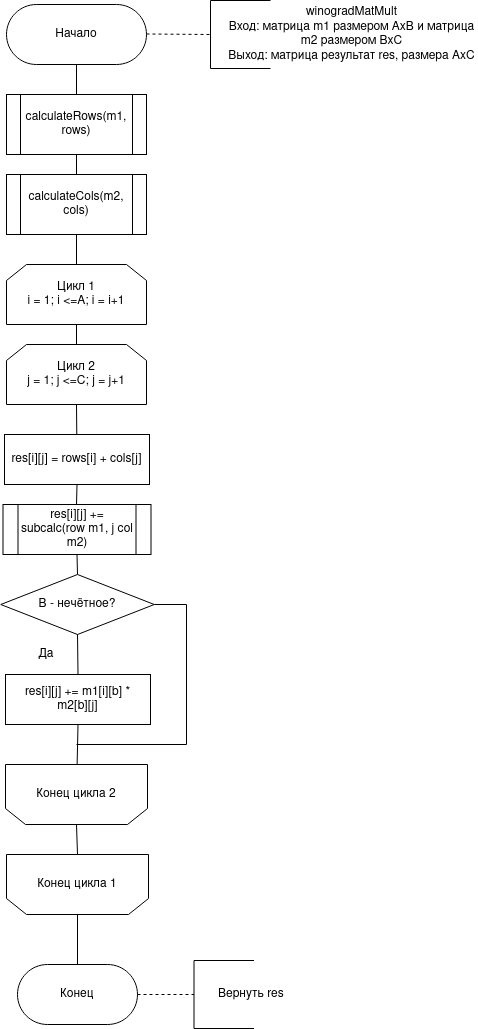
\includegraphics[height=0.65\textheight]{sem-v-aa-master/lab1/tex/inc/schemes/winograd_0.drawio.png}
    \caption{Схема стандратного умножения матриц}
    \label{fig:simple}
\end{figure}

\begin{figure}
    \caption{Схемы алгоритма Копперсмита---Винограда}
    \centering
    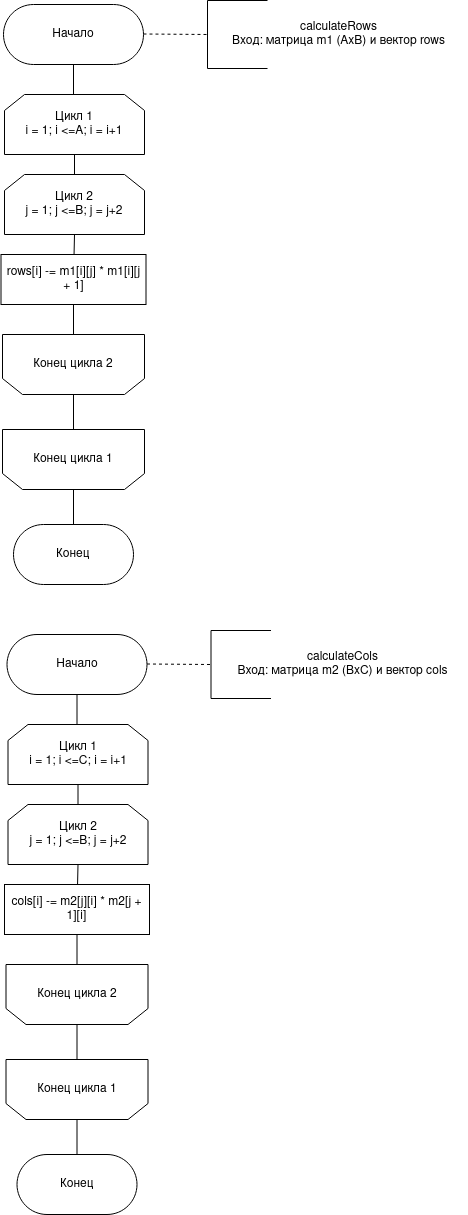
\includegraphics[height=0.8\textheight]{sem-v-aa-master/lab1/tex/inc/schemes/winograd_1.drawio.png}
    \label{fig:wino}
\end{figure}

\section{Модель вычислений}

Для последующего вычисления трудоемкости введем модель вычислений:
\begin{enumerate}[1.]
    \item Операции из списка \ref{eq:operations} имеют трудоемкость $1$. 
    \begin{equation}
        +,-,/,\%,=,\ne,<,>,\leq,\geq,[\;],++,--
        \label{operations}
    \end{equation}
    \item Трудоемкость условного оператора расчитвыается как \ref{eq:conditional}
    \begin{equation}
        f_{if} = f_{условия} + 
        \begin{cases}
            f_{A},& \text{если условие выполняется},\\
            f_{B},& \text{иначе}.
        \end{cases}
        \label{eq:conditional}
    \end{equation}
    \item Трудоемкость цикла рассчитывается как \ref{eq:loop}
    \begin{equation}
        f_{\text{цикл}} = f_{\text{сравнения}} + N \cdot (f_{\text{тела}} + f_{\text{инкремента}} + f_{\text{сравнения}})
        \label{eq:loop}
    \end{equation}
    \item трудоемкость вызова функции равно $0$.
\end{enumerate}

\section{Трудоемкость алгоритмов}
\subsection{Стандартный алгоритм умножения матриц}
Трудоемкость стандартного алгоритма умножения матриц состоит из:
\begin{itemize}
    \item внешнего цикла по $i \in [1..A]$, трудоемкость которого равна \\$f = 2 + A \cdot (2 + f_{\text{body}})$;
    \item Цикла по $j \in [1..C]$, трудоемкость которого равна $f = 2 + C \cdot (2 + f_{\text{body}})$;
    \item Скалярного умножения двух векторов -- цикл по $k \in [1..B]$, трудоемкость которого равна $f = 2 + 10 \cdot B$;
\end{itemize}
Трудоескость стандартного алгоритма равна трудоемкости внешнего цикла, можно вычислить ее, подставив циклы тела \ref{eq:outer_loop}:
\begin{equation}
    f_{\text{base}} = 2 + A \cdot (4 + C \cdot (4 + 10 \cdot B)) = 2 + 4 \cdot A + 4 \cdot A \cdot C + 10 \cdot ABC \approx 10 \cdot ABC
    \label{eq:outer_loop}
\end{equation}

\subsection{Алгоритм Копперсмита--Винограда}
Трудоемкость алгоритма Копперсмита--Винограда состоит из:
\begin{enumerate}[1.]
    \item Создание векторов строк и столбцов \ref{eq:vec}:
    \begin{equation}
        f_{\text{create}} = A + C
        \label{eq:vec}
    \end{equation}
    \item Заполнение вектора строк \ref{eq:rows}:
    \begin{equation}
        f_{\text{rows}} = 3 + \frac{B}{2} \cdot (5 + 12A)
        \label{eq:rows}
    \end{equation}
    \item Заполнение вектора столбцов \ref{eq:cols}:
    \begin{equation}
        f_{\text{cols}} = 3 + \frac{B}{2} \cdot (5 + 12C)
        \label{eq:cols}
    \end{equation}
    \item Цикла заполнения матрицы для четных размеров \ref{eq:loop}:
    \begin{equation}
        f_{\text{loop}} = 2 + A \cdot (4 + C \cdot (11 + \frac{25}{2} \cdot B))
        \label{eq:loop}
    \end{equation}
    \item Цикла, для дополнения умножения суммой последних нечетных строки и столбца, если общий размер нечетный. \ref{eq:last}:
    \begin{equation}
        f_{\text{last}} = \begin{cases}
            2,& \text{четная},\\
            4 + A \cdot (4 + 14C),& \text{нечетная}.
        \end{cases}
        \label{eq:last}
    \end{equation}

\end{enumerate}

Тогда для худшего случая -- то есть нечетного размера матрицы:
\begin{equation}
    f_{\text{worst}} = A + C + 12 + 8A + 5B + 6CB + 25AC + 12,5 \cdot ABC \approx \cdot 12,5ABC.
\end{equation}
Для случая с четным размером получаем \ref{eq:best}:
\begin{equation}
    f_{\text{best}} = A + C + 10 + 4A + 5B + 6CB + 11AC + 12,5ABC \approx 12,5ABC.
    \label{eq:best}
\end{equation}

\subsection{Оптимизированный алгоритм Копперсмита -- Винограда}
Трудоемкость улучшенного алгоритма Копперсмита -- Винограла состоит из: 
\begin{enumerate}[1.]
    \item создание векторов строки и столбцов \ref{eq:op_init}
    \begin{equation}
        f_{\text{init}} = A + C
        \label{eq:op_init}
    \end{equation}
    \item заполнение вектора строки \ref{eq:op_rows_init}
    \begin{equation}
        f_{\text{rows}} = 2 + \frac{B}{2}\cdot(4+8A)
        \label{eq:op_rows_init}
    \end{equation}
    \item заполнение вектора столбцов \ref{eq:op_cols_init}
    \begin{equation}
        f_{\text{cols}} = 2 + \frac{B}{2}\cdot(4+8A)
        \label{eq:op_cols_init}
    \end{equation}
    \item Цикла заполнения матрицы для четных размеров \ref{eq:op_loop_fill}
    \begin{equation}
        f_{\text{loop}} = 2 + \frac{B}{2}\cdot(4+8A)
        \label{eq:op_loop_fill}
    \end{equation}
    \item Цикла для дополнения умножения суммой последней нечетной строки и столбца (в случае нечетной размерности) \ref{eq:con_odd}
    \begin{equation}
        f_last = 3 + \begin{cases}
            0,& \text{четная},\\
            2 + 4 \cdot A + 13 \cdot nm \cdot (4 + 14C),& \text{нечетная}.
        \end{cases}
    \end{equation}
\end{enumerate}

Итого, для худшего случая и лучшего случая: 
\begin{equation}
    f_\text{winograd} = A + C + 10 + 4B + 4BC + 4BA + 8A + 20AC + 9ABC \approx 9ABC.
\end{equation}


\subsection{Структуры данных}
Для матрицы использовалась структура данных с тремя полями: количество строк, столбцов и данные матрицы.

\subsection{Тестирование}
Тестирование будет проведено на двух классах эквивалентности: матриц с четным размером и матриц с нечетным размером. 

\section{Вывод}

Основываясь на теоретическом материале, описанном в аналитическом разделе, были построены схемы обоих алгоритмов умножения матриц. Также были оценены их трудоемкости для лучших и худших случаев.

%%% Local Variables:
%%% mode: latex
%%% TeX-master: "rpz"
%%% End:

\chapter{Технологический раздел}
\label{cha:impl}

В данном разделе приведены требования к программному обеспечению, средства реализации и листинги кода. 

\section{Средства реализации}
Основным средством реализации в данной лабораторной работе является язык программирования C++17 \cite{iso_2017} ввиду своей высокой скорости работы и большого инструментария библиотек для анализирования программного обеспечения. Программное обеспечение было реализована при помощи структурного программирования.

\section{Требования к программному обеспечению}
Входнымы данными являются:
\begin{itemize}
    \item размерность массива $\text{size}$;
    \item $\text{size}$ однотипных элементов массива $\text{arr}$.
\end{itemize}
Выходными данными получается отсортированный массив $\text{arr}$.



\section{Реализации алгоритмов}

\begin{lstlisting}[caption=Алгоритм поразрядной сортировки]
void radix_ui(register unsigned int vector[], register const unsigned int size) {

    const int MAX_UINT__ = ((((1 << ((sizeof(unsigned int) << 3) - 2)) - 1) << 1) + 1);
    const int LAST_EXP__ = (sizeof(unsigned int) - 1) << 3;
    
#define PRELIMINARY__ 100
#define MISSING_BITS__ exp < (sizeof(unsigned int) << 3) && (max >> exp) > 0
#define LOOP_MAX__(a, b)				\
    for(s = &vector[a], k = &vector[b]; s < k; ++s) {	\
	if(*s > max)  {					\
	    max = *s;					\
	}						\
    }
    \end{lstlisting}
    \begin{lstlisting}[caption=Алгоритм поразрядной сортировки]
    register unsigned int *b, *s, *k;
    register unsigned int exp = 0;
    register unsigned int max = exp;

    unsigned int i, *point[0x100];
    int swap = 0;
    
    const unsigned int preliminary = (size > PRELIMINARY__) ? PRELIMINARY__ : (size >> 3);
    

    LOOP_MAX__(1, preliminary);
    if(max <= (MAX_UINT__ >> 7)) {	
	LOOP_MAX__(preliminary, size);
    }
    
    b = (unsigned int *)malloc(sizeof(unsigned int) * size);
    
#define SORT_BYTE__(vec, bb, shift)					\
    unsigned int bucket[0x100] = {0};					\
    register unsigned char *n = (unsigned char *)(vec) + (exp >> 3),*m; \
    for(m = (unsigned char *)(&vec[size & 0xFFFFFFFC]); n < m;) {	\
	++bucket[*n]; n += sizeof(int);					\
	++bucket[*n]; n += sizeof(int);					\
	++bucket[*n]; n += sizeof(int);					\
	++bucket[*n]; n += sizeof(int);					\
    }									\
    for(n = (unsigned char *)(&vec[size & 0xFFFFFFFC]) + (exp >> 3),	\
	    m = (unsigned char *)(&vec[size]); n < m;) {		\
	++bucket[*n]; n += sizeof(int);					\
    }									\
    s = bb;								\
    int next = 0;							\
    for(i = 0; i < 0x100; ++i) {					\
	if(bucket[i] == size) {						\
	    next = 1;							\
	    break;							\
	}								\
    }									\
    if(next) {								\
	exp += 8;							\
	continue;							\
    }									\
    \end{lstlisting}
\begin{lstlisting}[caption=Алгоритм поразрядной
    for(i = 0; i < 0x100; s += bucket[i++]) {				\
	point[i] = s;							\
    }									\
    for(s = vec, k = &vec[size]; s < k; ++s) {	\

	*point[(*s shift) & 0xFF]++ = *s;				\
    }									\
    swap = 1 - swap;							\
    exp += 8;
    
    /* Sort each byte (if needed) */
    while(MISSING_BITS__) {
	if(exp) {
	    if(swap) {
		SORT_BYTE__(b, vector, >> exp);
	    } else {
		SORT_BYTE__(vector, b, >> exp);
	    }
	} else {
	    SORT_BYTE__(vector, b, );
	}
    }

    if(swap) {
	memcpy(vector, b, sizeof(unsigned int) * size);
    }
    
    free(b);
    
#undef PRELIMINARY__
#undef MISSING_BITS__
#undef LOOP_MAX__
#undef SORT_BYTE__
\end{lstlisting}

\begin{lstlisting}[caption=Алгоритм пирамидальной сортировки]
void max_heapify(int a[], int i, int n)
{
  int l,r,largest,loc;
  l=2*i;
  r=(2*i+1);
  if((l<=n)&&a[l]>a[i])
    largest=l;
  else
      \end{lstlisting}
\begin{lstlisting}[caption=Алгоритм пирамидальной сортировки]
    largest=i;
  if((r<=n)&&(a[r]>a[largest]))
    largest=r;
  if(largest!=i)
    {

      loc=a[i];
      a[i]=a[largest];
      a[largest]=loc;
      MAX_HEAPIFY(a, largest,n);
    }
}
void BUILD_MAX_HEAP(int a[], int n)
{
  for(int k = n/2; k >= 1; k--)
    {
      max_heapify(a, k, n);
    }
}
void heap_sort(int a[], int n)
{

  BUILD_MAX_HEAP(a,n);
  int i, temp;
  for (i = n; i >= 2; i--)
    {
      temp = a[i];
      a[i] = a[1];
      a[1] = temp;
      max_heapify(a, 1, i - 1);
    }
}
\end{lstlisting}
\newpage
\begin{lstlisting}[caption=алгоритм пузырьковой сортировки]
      void bubbleSort(vector <int> &v, int n) {
	bool swapped = true;
	int i = 0;

	while (i < n - 1 && swapped) {
		swapped = false;
		
		for (int j = n - 1; j > i; j--) { // unordered part
			
			if (v[j] < v[j - 1]) {
				swap(v[j], v[j - 1]);
				swapped = true;
			}
		}
		i++;
	}
}
\end{lstlisting}
 
\section{Вывод}

В данном разделе были разработаны исходный код всех трех алгоритмов: порразрядной сортировки, пирамидальной сортировки и сортировки пузырьком. 

%%% Local Variables:
%%% mode: latex
%%% TeX-master: "rpz"
%%% End:

\chapter{Исследовательский раздел}
\label{cha:research}

\section{Пример работы}

\section{Технические характеристики}

\section{Время выполнения}

\section{Использование памяти}

%%% Local Variables:
%%% mode: latex
%%% TeX-master: "rpz"
%%% End:


\backmatter
            
\Conclusion % заключение к отчёту

В результате проделанной работы стало ясно, что ничего не ясно...

%%% Local Variables: 
%%% mode: latex
%%% TeX-master: "rpz"
%%% End: 
%% заключение


% % Список литературы при помощи BibTeX
% Юзать так:
%
% pdflatex rpz
% bibtex rpz
% pdflatex rpz

\bibliographystyle{ugost}
\bibliography{rpz}
%%% Local Variables: 
%%% mode: latex
%%% TeX-master: "rpz"
%%% End: 



\end{document}

%%% Local Variables:
%%% mode: latex
%%% TeX-master: t
%%% End:
